% LaTeX source for book ``代数学方法'' in Chinese
% Copyright 2018  李文威 (Wen-Wei Li).
% Permission is granted to copy, distribute and/or modify this
% document under the terms of the Creative Commons
% Attribution 4.0 International (CC BY 4.0)
% http://creativecommons.org/licenses/by/4.0/

% To be included
\chapter{Markov链}

\begin{compactitem}
	\item Markov性,转移概率和转移矩阵.
	\item C-K方程.
	\item 常返性和周期性.
	\item 平稳分布与极限分布.
	\item Markov微分方程.
\end{compactitem}

\section{基本概念}\label{sec:BisCon}

\begin{definition}\label{def:Markov}\index{Markovlian@Markov链 (Markov Chain)}
	随机过程\(\{X_n,n=0,1,2,\cdots\}\)称为\emph{Markov链},如果如果它只取有限个或可列个值,并且对任意的\(n\geqslant 0\),以及任意状态\(i,j,i_0,i_1,\cdots,i_{n-1}\),有
	\begin{align*}
		  & P\{X_{n+1}=j|X_n=i,X_{n-1}=i_{n-1},\cdots,X_1=i_1,X_0=i_0\} \\
		= & P\{X_{n+1}=j|X_n=i\}
	\end{align*}
	式中,\(X_n=i\)表示过程在时刻\(n\)处于状态\(i\),称\(\{0,1,2,\cdots\}\)为该过程的状态空间,记为S。
\end{definition}

上式刻画了Markov链的特性,称为Markov性。对Markov链。给定过去的状态\(X_0,X_1,\cdots,X_{n-1}\)以及现在的状态\(X_n\),将来的状态\(X_{n+1}\)的条件分布与过去的状态独立,只依赖于现在的状态。

\begin{definition}\label{def:ProbTran}\index{zhuanyigailv@转移概率 (Probability of Transfer)}
	条件概率\(P\{X_{n+1}=j|X_n=i\}\)为Markov链\(\{X_n,n=0,1,2,\cdots\}\)的一步转移概率,简称\emph{转移概率},记为\(p_{ij}\),它代表处于状态\(i\)的过程下一步转移到状态\(j\)的概率。
\end{definition}

一般情况下,转移概率与状态\(i,j\)和时刻\(n\)有关。

\begin{definition}\label{def:TimIndMarkov}\index{shiqimarkovlian@时齐Markov链 (Time Independent Markov Chain)}
	当Markov链的转移概率\(p_{ij}=P\{X_{n+1}=j|X_n=i\}\)只与状态\(i,j\)有关,而与时刻\(n\)无关时,称为
	\emph{时齐Markov链};否则,称为非时齐的Markov链。
\end{definition}

\begin{definition}\label{def:TransMatr}\index{zhuanyijuzhen@转移矩阵 (Transfer matrix)}
	通常将\(p_{ij},i,j\in S\)排成一个矩阵的形式,\(\mathbf{P}=(p_{ij})\)。称为状态转移矩阵,或简称\emph{转移矩阵}。
\end{definition}

转移概率具有如下性质:
\begin{enumerate}[\bfseries (1)]
	\item \(p_{ij}\geqslant 0,i,j\in S\);
	\item \(\sum_{j\in S}p_{ij}=1,\forall i\in S\).
\end{enumerate}

\section{C-K方程}

\begin{definition}\label{def:nTransMatr}\index{nbuzhuanyijuzhen@n步转移矩阵 (N-Step Transfer matrix)}
	称条件概率
	\begin{align*}
		p_{ij}^{(n)}=P\{X_{m+n}=j|X_m=i\},\quad i,j\in S;m \geqslant 0; n\geqslant 1
	\end{align*}
	为Markov链的n步转移概率,相应地称\(\mathbf{P}^{(n)}=(p_{ij}^{(n)})\)为\emph{\(n\)步转移概率矩阵}。
\end{definition}

\(n\)步转移概率\(p_{ij}^{(n)}\)指的是系统从状态\(i\)经过\(n\)步后转移到状态\(j\)的概率,
它对中间的\(n-1\)步转移经过的状态无要求,也有可能已经经过了状态\(j\)。


\begin{theorem}[Chapman-Kolmogorov方程,简称C-K方程]\label{prop:C-K}
	对一切\(n,m\geqslant0,i,j\in S\)有
	\begin{enumerate}[\bfseries (1)]
		\item \(p_{ij}^{(m+n)}=\sum_{k\in S}p_{ik}^{(m)}p_{kj}^{(n)}\);
		\item \(\mathbf{P}^{(n)}=\mathbf{P}\cdot \mathbf{P}^{(n-1)}=\mathbf{P}\cdot \mathbf{P}\cdot \mathbf{P}^{(n-2)}=\cdot =\mathbf{P}^{n}\).
	\end{enumerate}
\end{theorem}

仅证明定理\ref{prop:C-K}(1)。

\begin{proof}
	\begin{align*}
		p_{ij}^{(m+n)}
		 & =P\{X_{m+n}=j|X_0=i\}                                       \\
		 & =\frac{P\{X_{m+n}=j,X_0=i\}}{P\{X_0=i\}}                    \\
		 & =\sum_{k\in S}\frac{P\{X_{m+n}=j,X_m=k,X_0=i\}}{P\{X_0=i\}} \\
		 & =\sum_{k\in S}\frac{P\{X_{m+n}=j,X_m=k,X_0=i\}}{P\{X_0=i\}}
		\cdot\frac{P\{X_m=k,X_0=i\}}{P\{X_m=k,X_0=i\}}                 \\
		 & =\sum_{k\in S} P\{X_{m+n}=j|X_m=k,X_0=i\}P\{X_m=k|X_0=i\}   \\
		 & =\sum_{k\in S}p_{ik}^{(m)}p_{kj}^{(n)}
	\end{align*}
\end{proof}

\section{Markov链的状态分类与性质}

\begin{definition}\label{def:IntPer}\index{zhuangtaihutong@状态互通(Interoperability of states)}
	若存在\(n\geqslant 0\)使得\(p_{ij}^{(n)}\),称状态\(i\)可达状态\(j(i,j\in S)\),记为\(i\rightarrow j\)。若同时有\(j\rightarrow i\),则称\(i\)与\(j\)\emph{互通},记为\(i\leftrightarrow j\)。
\end{definition}

互通是一种等价关系,它具有:
\begin{enumerate}[\bfseries (1)]
	\item 自返性:\(i\leftrightarrow i\);
	\item 对称性:\(i\leftrightarrow j\),则\(j\leftrightarrow i\);
	\item 传递性:\(i\leftrightarrow j,j\leftrightarrow k\),则\(i\leftrightarrow k\)。
\end{enumerate}

所以可以将两种互通状态归为一类,在同一类的状态都是互通的,而且任何一种状态不能同时属于两个不同的类。

\begin{definition}\label{def:Reducible}\index{keyue@可约(Reducible)}
	若Markov链只存在一个类,就称它是\textbf{不可约的};否则称为\emph{可约的}。
\end{definition}

\begin{definition}\label{def:Period}\index{zhouqi@周期(Period)}
	若集合\(\{n:n\geqslant 1,p_{ii}^{(n)}>0\}\)非空,则称它的最大公约数\(d=d(i)\)为状态\(i\)的\emph{周期}。若\(d>1\),则称\(i\)是周期的;若\(d=1\),则称\(i\)是非周期的。此外规定,集合\(\{n:n\geqslant 1,p_{ii}^{(n)}>0\}\)为空集时,周期为无穷大。
\end{definition}

周期的含义不是\(d\)步内就能回到初始状态,而是当步数足够大时,每过\(d\)步都有可能回到初始状态。属于同一类的状态周期相同。

\begin{definition}\label{def:ConRet}\index{changfanzhuangtaiyufeichangfanzhuangtai@常反状态与非常返状态(Constant Return and Unonstan Return)}
	对任何状态i,j,以\(f_{ij}^{(n)}\)记从i出发经过n步后首次到达j的概率,则有
	\begin{align*}
		f_{ij}^{(n)} & =\delta_{ij}                                              \\
		f_{ij}^{(n)} & =P\{X_n=j,X_k\neq j,k=1,2,\cdots,n-1|X_0=i\},n\geqslant 1
	\end{align*}
	令\(f_{ij}=\sum_{n=1}^{\infty}f_{ij}^{(n)}\),若\(f_{jj}=1\),则称状态\(j\)为\emph{常返状态};若\(f_{jj}<1\),则称状态\(j\)为\emph{非常返状态}。
\end{definition}

\(f_{ij}^{(n)}\)表示首次到达的概率,所以\(f_{ij}^{(n)}\leqslant p_{ij}^{(n)}\)。\(f_{jj}\)表示所有从\(j\)出发,经过有限步,首次回到\(j\),且不路经\(j\)的概率之和。当\(i\)为常返状态时,从\(i\)出发,在有限步内将以概率1返回状态\(i\);当\(i\)为非常返状态时,过程以概率\(1-f_{ii}>0\)不再返回到\(i\)。

\begin{definition}\label{def:numret}{正常返状态与零常返状态}
	对于\underline{常返状态\(i\)},定义
	\begin{align*}
		\mu_i=\sum_{n=1}^{\infty}nf_{ii}^{(n)}
	\end{align*}
	,表示的是由\(i\)出发再返回到\(i\)所需的平均步数(时间)。若\(\mu_i<+\infty\),则称\(i\)为\emph{正常返状态};若\(\mu_i=+\infty\)则称\(i\)为\emph{零常返状态}。
\end{definition}

要根据转移概率矩阵对状态进行分类,需要按照如下步骤:(1)画出状态转移图;(2)分析状态的分类与互通性;(3)计算各个状态分类的周期;(4)分析常返性。

\begin{theorem}\label{prop:unconretproptran}
	状态\(i\)为常返状态当且仅当\(\sum_{n=0}^{\infty}p_{ii}^{(n)}=\infty\),为非常返时有\(\sum_{n=0}^{\infty}p_{ii}^{(n)}=\frac{1}{1-f_{ii}}\)
\end{theorem}

注意到\(\frac{1}{1-f_{ii}}=\sum_{i=o}^{\infty}(f_{ii})^n\)。

\section{极限定理与平稳分布}

Markov链的某些概念——例如零常返状态和周期的定义——不够直观,其中的内涵不容易区分,造成了理解上的困难。这时需要考虑到,实际案例中考察的Markov链大多不知何时开始,也不知何时结束,例如某个生态系统中种群的数量变化。这时假设系统时间足够长,初始状态的影响可以忽略,是十分合理的。

考察Markov链大多是考虑其长期性质,这个角度对理解markov链的概念、分类和性质十分有用。这节内容就是考虑当步数(时间)n足够大时,Mrkov链的某些性质。

\begin{theorem}\label{prop:conretproptran}
	若状态\(i\)是周期为\(d\)的常返状态,则
	\begin{align*}
		\lim_{n\to \infty}p_{ii}^{(nd)}=\frac{d}{\mu_i}
	\end{align*}
	当\(\mu_i=\infty\)时,\(\frac{d}{\mu_i}=0\)。
\end{theorem}

首先回忆一下常返状态的概念:若\(f_{ii}=\sum_{n=1}^{\infty}f_{ii}^{(n)}=1\),则称为状态\(i\)为常返状态时,若\(f_{ii}<1\),则称态\(i\)为非常返状态或瞬过状态。其中\(f_{ii}^{(n)}\)为从\(i\)出发经过\(n\)步后首次达到\(i\)的概率,那么\(f_{ii}\)就表示从\(i\)出发达到\(i\)的概率。首次达到的条件限制了,如果某条路径重复经过状态\(i\),只记第一次。常返状态中\(f_{ii}=1\),代表从\(i\)出发必然会回到\(i\),因此称为\textbf{常返}。

再回忆一下状态互通的概念:若存在\(n\geqslant 0\)使得\(p_{ij}^{(n)}\),称状态\(i\)可达状态\(j(i,j\in S)\),记为\(i\rightarrow j\)。若同时有\(j\rightarrow i\),则称\(i\)与\(j\)互通,记为\(i\leftrightarrow j\)。互通的状态可归为一类。状态互通意味着,在有限步内,从\(i\)出发可以达到\(j\)或从\(j\)出发可以达到\(i\)。如果这时状态\(i\)时一个常返状态,那么状态\(j\)是常返状态吗?答案是肯定的,见课本上关于常返是一个类性质的证明。

这时再看常返状态状态转移概率的极限。周期\(d\)的含义是所有从\(i\)回到\(i\)的路径长度的最大公约数。
当步数足够大时,所有从\(i\)回到\(i\)的路径都有可能经过,且不止经过了一次,这时已经不能区分从哪条路径回到\(i\),但每过\(d\)步,都有可能回到\(i\),这就是取最大公约数的原因,也是周期的含义。每过\(d\)步都有可能回到\(i\),那么这个可能的概率是多少?定理\ref{prop:conretproptran}给出了。

\(\lim_{n\to \infty}p_{ii}^{(nd)}\)即为当\(n\)足够大时,每经过\(d\)步,回到状态\(i\)的概率。\(\mu_i=\sum_{n=1}^{\infty}nf_{ii}^{(n)}\)表示从\(i\)出发回到状态\(i\)的平均步数。那么经过\(d\)步,回到状态\(i\)的概率就是\(\frac{d}{\mu_i}\)。

对于周期为\(d\)的常返状态,可以不可以说,当\(n\)足够大时,每步都有\(\frac{1}{\mu_i}\)的概率回到状态\(i\)呢?当\(d=1\)时,这种说法是正确的,但当周期不为1时,不一定每步都有可能回到状态\(i\),\(\lim_{n\to \infty}p_{ii}^{(nd)}\)中的\((nd)\)限制了这一点。

对于非常返状态,即\(f_{ii}<1\),从\(i\)出发不一定能够回到\(i\)。这里容易存在误解的地方是,从\(i\)出发,要么能够回到\(i\),要么不能够回到\(i\),所以对于非常返状态,\(f_{ii}=0\)。
这种误解产生的原因是,默认若\(p_{ij}>0\),则\(p_{ji}>0\)。一般情况下,这个条件不一定能够满足,有些状态之间转移是单向的。经过这样的转移之后,无法原路径返回,也不存在其他状态之间的转移方式,再回到原来状态,这也是非常返状态也称为瞬过状态的原因。那么当\(n\)足够大时,\(\lim_{n\to \infty}p_{ii}^{(n)}=0\),这由级数\(\sum_{n=0}^{\infty}p_{ii}^{(n)}=\frac{1}{1-f_{ii}}\)有限也可以推出。

\begin{definition}\label{defi:limdis}
	如果所有状态相同且均是周期为1的正常返状态,则称Markov链是遍历的。对于遍历的Markov链,极限
	\begin{align*}
		\lim_{n\to \infty}p_{ij}^{(n)}=\pi_j,\quad j\in S
	\end{align*}
	称为Markov链的\emph{极限分布}。
\end{definition}

极限分布就是平稳分布,且是唯一的平稳分布。

结合平稳方程的概念,需要通过解方程\(\boldsymbol{\pi}\mathbf{P}=\boldsymbol{\pi}\),或
\(\boldsymbol{\pi}(\mathbf{P}-\mathbf{I})=\mathbf{0}\)来求极限分布。需要注意的是,方程\(\boldsymbol{\pi}(\mathbf{P}-\mathbf{I})=\mathbf{0}\)不同于线性方程组的表示\(\mathbf{Ax}=\mathbf{b}\),这里\(\boldsymbol{\pi}\)是行向量,而线性方程组的解\(\mathbf{x}\)通常用列向量表示。这里\(\boldsymbol{\pi}\)是左乘,而不是右乘。

由于状态转移矩阵的性质\((2)\sum_{j\in S}p_{ij}=1,\forall i\in S\),\(\mathbf{P}\)并不是列满秩的,额外限定\(\sum_{j\in S}\pi_{j}=1,\forall j\in S\),即可求出\(\boldsymbol{\pi}\)。

\section{连续时间Markov链}

连续时间Markov链的状态空间仍然是离散的,但是时间是连续变化的。

\begin{definition}\label{def:contimemarkov}\index{lianxushijianmarkovlian@连续时间Markov链(Continuous Time Markov Chain)}
	过程\(\{X(t),t\geqslant 0\}\)的状态空间S为离散空间,通常设S为\(\mathbb{Z^+}\)或其子集。若\(\forall s,t\geqslant 0\)以及\(i,j\in S\),有
	\begin{align*}
		  & P\{X(t+s)=j|X(s)=i,X(u)=x(u),0\leqslant u<s\} \\
		= & P\{X(t+s)=j|X(s)=j\}
	\end{align*}
	成立,则称\(\{X(t),t\geqslant 0\}\)是一个\emph{连续时间Markov链}。
\end{definition}

条件概率\(P\{X(t+s)=j|X(s)=i\}\)记作\(p_{ij}(s,t)\),表示过程在时刻\(s\)处于状态\(i\),经过\(t\)时间后转移到\(j\)的转移概率,\(\mathbf{P}(s,t)=(p(s,t))\)为相应的转移概率矩阵。

\begin{definition}\label{def:TimIndConMarkov}\index{shiqimarkovlian@时齐Markov链(Time Independent Continuous Markov Chain)}
	若\(p_{ij}\)与s无关,则称连续时间Markov链是\emph{时齐}的。简记为\(p_{ij}(s,t)=p_{ij}(t)\),相应的\(\mathbf{P}(t)=(p_{ij}(t))\)。
\end{definition}

在没有特别指出时,通常都指时齐Markov链。

\begin{theorem}\label{prop:ConMarkovDis}
	设\(\{X(t),t\geqslant 0\}\)是连续时间Markov链,假定在时刻0过程刚刚到达状态\(i(i\in S)\)。记\(\tau_i\)为过程在离开状态\(i\)之前在状态i停留的时间,则\(\tau_i\)服从指数分布。
\end{theorem}

回忆2.3节与Possion过程相联系的分布。\(X_n\)表示第\(n\)次时间与第\(n+1\)次事件发生的间隔,则\(X_n\)服从参数为\(\lambda\)的指数分布且相互独立。那么Poisson过程是连续时间Markov链吗?是的。因此可以用Poisson过程的结论来理解连续时间Markov链。

\begin{theorem}\label{prop:ConMarkovC-K}
	连续时间Markov链的转移概率\(p_{ij}(t)\)满足:
	\begin{enumerate}[\bfseries (1)]
		\item \(p_{ij}\geqslant 0\);
		\item \(\sum_{i\in S}p_{ij}=1\);
		\item \(p_{ij}(t+s)=\sum_{k\in S}p_{ik}(t)p_{kj}(s)\).
	\end{enumerate}
\end{theorem}

定理\ref{prop:ConMarkovC-K}(3)通常称为连续时间Markov链的C-K方程。

\begin{theorem}[跳跃强度]\label{prop:jumpstre}
	\begin{enumerate}[\bfseries (1)]
		\item \(\lim_{t\to 0}\frac{1-p_{ii}(t)}{t}=q_{ii}\leqslant \infty\);

		\item \(\lim_{t\to 0}\frac{p_{ij}(t)}{t}=q_{ij}< \infty\).
	\end{enumerate}
\end{theorem}

在(1)中,\(i\)时间内,从状态\(i\)转移到另一个状态的转移概率为\(1-p_{ii}(t)\),\(q_{ii}\)称为跳跃强度,表示离开状态\(i\)的强度。在(2)中,\(p_{ij}(t)\)表示t时间内,从状态\(i\)转移到状态\(j\)的概率,\(q_{ij}\)则表示从状态\(i\)转移到状态\(j\)的强度(或理解为单位时间发生的概率)。由\(1-p_{ii}(t)\)和\(p_{ij}(t)\)的含义可知
\begin{align*}
	q_{ii}=\sum_{j\neq j}q_{ij}<+\infty
\end{align*}

\begin{theorem}[Kolmogorov微分方程]\label{prop:KolmogorovDifEqu}
	\(\forall i,j\in S,t\geqslant 0\)且\(\sum_{j\neq i}q_{ij}=q_{ii}<+\infty\),有
	\begin{enumerate}[\bfseries (1)]
		\item 后向方程
		      \begin{align*}
			      p'_{ij}(t)=\sum_{k\neq i}q_{ik}p_{kj}(t)-q_{ii}p_{ij}(t)
		      \end{align*}
		\item 在适当的正则条件下,有前向方程
		      \begin{align*}
			      p'_{ij}(t)=\sum_{k\neq j}q_{kj}p_{ik}(t)-q_{jj}p_{ij}(t)
		      \end{align*}
	\end{enumerate}
\end{theorem}

下面仅解释如何理解\textbf{前向方程}:结合对跳跃强度\ref{prop:jumpstre}的理解,\(q_{kj}p_{ik}(t)\)是(从状态\(i\)转移到状态\(j\)的概率)乘以(从状态\(k\)转移到状态\(j\)的强度),它表示从状态\(i\)通过状态\(k(k\neq j)\)再转移到状态\(j\)的强度。求和\(\sum_{k\neq j}q_{kj}p_{ik}(t)\)表示从所有其他状态转移到状态\(j\)的强度之和,即表示状态\(j\)\textbf{增加}的强度。\(q_{jj}p_{ij}(t)\)是转移离开状态\(j\)的强度乘以从状态\(i\)转移到状态\(j\)的概率,表示从状态\(i\)转移到状态\(j\)再转移离开状态\(j\)的强度。那么\(q_{kj}p_{ik}(t)-q_{jj}p_{ij}(t)\)就表示从状态\(i\)转移到状态\(j\)的强度,即\( p'_{ij}(t)\)。

关于为何,从状态\(i\)转移到状态\(j\)再转移离开状态\(j\)的强度,是从状态\(i\)转移到状态\(j\)的概率乘以转移离开状态\(j\)的强度,而不是转移离开状态\(i\)的强度乘以从状态\(i\)转移到状态\(j\)的概率。因为这个方程称为\textbf{前向方程},而不是\textbf{后向方程}。后向方程的含义可以对照理解。

\textbf{练习:}利用定理\ref{prop:KolmogorovDifEqu},证明由Poisson的第二个定义\ref{def:Pois-Proc2}可以推出第一个定义\ref{def:Pois-Proc}.

\newpage

\begin{Exercises}
	\item 有6个车站,车站中间的公路连接情况如图1所示。汽车每天可以从一个站驶向与之直接相邻的车站,并在夜晚达到车站留宿,次日凌晨重复相同的活动。设每天凌晨汽车开往临近的任何车站都是等可能的,试说明很长时间后,各车站每晚留宿的汽车比例趋于稳定。求出这个比例以便正确地设置各站的服务规模。
	\begin{figure}[h!]\label{fig:road}
		\begin{center}
			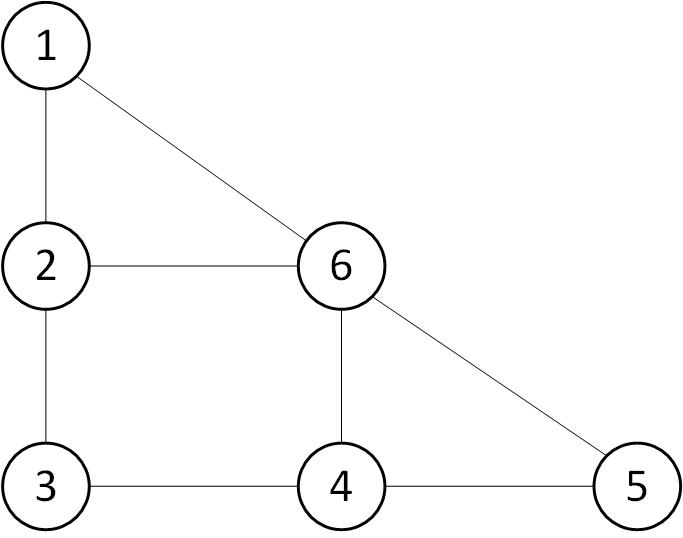
\includegraphics[width=0.3\textwidth]{fig1.jpg}
			\caption{车站之间公路连接情况}
		\end{center}\end{figure}

	\newpage
	\item 考察某一系统运作情况(如机器运转)。如果运作正常,则认为系统处于状态1;如果系统正在调整(例如机器维修,计算机杀毒等),则认为系统处于状态0。系统运作一段时间后,会遇到不能正常运作的情况,此时系统需要调整。调整后又恢复运作。假定系统从开始运作直到需要调整的运作时间是随机的,服从参数为\(\mu\)的指数分布,密度函数为\(\mu e^{-\mu t},t>0\)。而调整期也是随机的,服从参数为\(\lambda\)的指数分布,密度函数为\(\lambda e^{-\lambda t},t>0\)。假定运作周期是相互独立的,调整期也是相互独立的。如果令\(X(t)\)为系统在时刻\(t\)所处的状态,则由于在时刻\(t\)以后,系统所处的状态仅与在时刻\(t\)及其以后的剩余运作时间或剩余调整时间有关。利用指数分布的无记忆性知道,\(X(t)\)是时齐Markov链。利用Kolmogorov方程求出此Markov链的转移概率。
	\newpage
	\vspace{13em}
	\item 设今日有雨,则明日也有与的概率为0.7,今日无雨,明日有雨的概率为0.5。求星期一有雨,星期三也有雨的概率。
	\vspace{13em}
	\item 某人有\(r\)把伞用于上下班,如果一天的开始他在家(一天的结束他在办公室)中而且天下雨,只要有伞可取到,他将拿一把到办公室(家)中。如果天不下雨,那么他不带伞,假设每天的开始(结束)下雨的概率为\(p\),且与过去情况独立。
	\begin{enumerate}[\bfseries (1)]
		\item 定义一个有\(r+1\)个状态的Markov链并确定转移概率;
		\item 计算极限分布;
		\item 他被淋湿的平均次数所占比率是多少?(如果天下雨而全部伞在另一处,那么称他被淋湿)。
	\end{enumerate}
	\vspace{15em}
	\item 若\(f_{ii}<1,f_{jj}<1\),证明
	\begin{align*}
		 & \sum_{n=1}^{\infty}p_{ij}^{(n)}<+\infty                                            \\
		 & f_{ij}  =\frac{\sum_{n=1}^{\infty}p_{ij}^{(n)}}{1+\sum_{n=1}^{\infty}p_{jj}^{(n)}}
	\end{align*}
	\newpage

	\item 考虑有两个状态的连续时间Markov链,状态为0和1,链在离开0到达1之前在状态0停留的时间服从参数为\(\lambda\)的指数分布,相应地在1停留的时间是参数为\(\mu\)的指数变量。对此建立Markov微分方程,并求其解。
	\vspace{15em}
	\item 设有一质点在1,2,3上做随机跳跃,在时刻t它位于三点之一,且在\([t,t+h]\)内以概率\(\frac{1}{2}+o(h)\)分别可以跳到其他两个状态。试求状态概率满足的Kolmogorov方程。
\end{Exercises}